%!TEX root=ast2016.tex

\begin{figure*}[t]
  \centering
  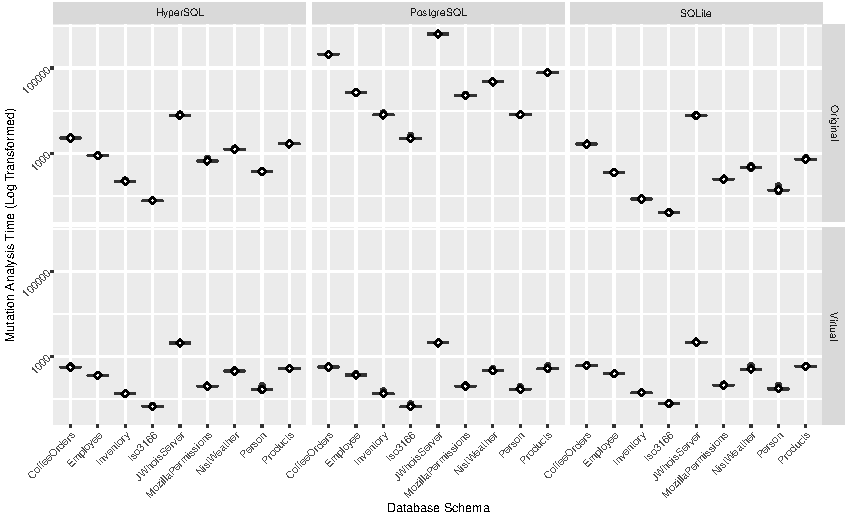
\includegraphics[scale=1.0]{graphics/graphic_bwplot_schema_analysistime_org_vm.pdf}
  \caption{Box plot of the execution time for the standard and virtual mutation analysis techniques.}
  \label{fig:graphic_bwplot_schema_analysistime_org_vm}

  % Details about the box plot from the R documentation:

  % The lower and upper "hinges" correspond to the first and third quartiles (the 25th and 75th percentiles). This differs
  % slightly from the method used by the boxplot function, and may be apparent with small samples. See boxplot.stats for for
  % more information on how hinge positions are calculated for boxplot.

  % The upper whisker extends from the hinge to the highest value that is within 1.5 * IQR of the hinge, where IQR is the
  % inter-quartile range, or distance between the first and third quartiles. The lower whisker extends from the hinge to
  % the lowest value within 1.5 * IQR of the hinge. Data beyond the end of the whiskers are outliers and plotted as points
  % (as specified by Tukey).

  {\small \justifying{ \noindent For a detailed description of the meaning of the boxes in this plot, please refer to
      Section~\ref{sec:experimental-setup}. The boxes in this plot are noticeably compressed because there is little variability in
      the timings across the different configurations.  Since the results from running the standard method on the
      \Postgres~DBMS differ substantially from those with the other techniques and databases, all of the
      data values were log-transformed, thereby best revealing the relevant trends.} \par}

  \vspace*{-1em}

\end{figure*}
